\documentclass[salesmen, twoside]{../../../templates/latex/2009/softproj}
\usepackage[english]{babel} % For a load of tiny changes in the text
\usepackage{graphicx, ctable, url, hyperref} % graphics, tables, urls and cross-referencing

\usepackage{amsmath}
\usepackage{eurosym}


\begin{document}
\begin{projdoc}

\chapter{Introduction}

\section{Purpose}
This document specifies the entire software architecture and design for the Salesmen software. These design decisions directly relate to the functionalities, performances, constraints, attributes and interfaces of the system, as they are mentioned in the Software Requirements Specification (SRS, \cite{SRS}) document.

\section{Scope}
This document describes the software architecture and design for the first stable release of the Salesmen software. The intended audience of this document exclusively includes the designers, the developers and the testers of the software.\\
It should be considered a thorough guide for the implementation of the software. However, developers may deviate from it as they see required during the implementation phase, as long as they discuss these changes with the design manager. 

\section{Reference materials}
See Appendix A.

\section{Definitions and acronyms \label{acronyms}}
\begin{tabular}{ll}
\textbf{CSS}   & Cascading Style Sheets \\
\textbf{EJB3}   & Enterprise Java Beans v3 \\
\textbf{HTML}   & Hypertext Markup Language \\
\textbf{XHTML}   & Extensible Hypertext Markup Language \\
\textbf{MVC}   & Model-View-Controller, a design pattern \\
\textbf{HQL}   & Hibernate Query Language \\
\textbf{J2EE}   & Java 2 Platform, Enterprise Edition \\
\textbf{JBoss}   & An application server \\
\textbf{RDBMS}    & Relational Database Management System \\
\textbf{SCMP}   & Software Configuration Management Plan \\
\textbf{SDD}    & Software Design Document \\
\textbf{SMTP}   & Single Mail Transfer Protocol \\
\textbf{SRS}    & Software Requirements Specification \\
\textbf{SQL}   & Structured Query Language \\
\end{tabular}

\chapter{System Architecture}
\section{Overview}
System architecture diagram: see Appendix B, \ref{fig_architecture}

\section{Three-Tier Architecture}
Three-tier architecture is a client-server architecture in which the user interface, functional process logic, computer data storage and data access are developed and maintained as independent modules, most often on separate platforms.

Apart from the usual advantages of modular software with well defined interfaces, the three-tier architecture is intended to allow any of the three tiers to be upgraded or replaced independently as requirements or technology change. For example, a change of operating system in the presentation tier would only affect the user interface code.

Typically, the user interface runs on a desktop PC or workstation and uses a standard graphical user interface, functional process logic may consist of one or more separate modules running on a workstation or application server, and a RDBMS on a database server or mainframe contains the computer data storage logic.

Three-tier architecture has the following three tiers:
\begin{itemize}
\item \textbf{Presentation tier}
This is the topmost level of the application. The presentation tier displays information related to such services as browsing merchandise, purchasing, and shopping cart contents. It communicates with other tiers by outputting results to the browser/client tier and all other tiers in the network.
\item \textbf{Application tier (Business Logic/Logic Tier)}
The logic tier is pulled out from the presentation tier and, as its own layer, it controls an application�s functionality by performing detailed processing.
\item \textbf{Data tier}
This tier consists of Database Servers. Here information is stored and retrieved. This tier keeps data neutral and independent from application servers or business logic. Giving data its own tier also improves scalability and performance. 
\end{itemize}

Benefits of using this architectural style include increased performance, flexibility, maintainability, reusability, and scalability.
\section{Discussion of Alternative Designs}
\textbf{MVC}
At first glance, the three tiers may seem similar to the MVC (Model View Controller) concept. However, topologically they are different. A fundamental rule in a three-tier architecture is the client tier never communicates directly with the data tier; in a three-tier model all communication must pass through the middleware tier. Conceptually the three-tier architecture is linear. However, the MVC architecture is triangular: the View sends updates to the Controller, the Controller updates the Model, and the View gets updated directly from the Model.

From a historical perspective the three-tier architecture concept emerged in the 1990�s from observations of distributed systems (e.g., web applications) where the client, middleware and data tiers ran on physically separate platforms. Whereas MVC comes from the previous decade and is based on observations of applications that ran on a single graphical workstation; MVC was applied to distributed applications much later in its history.


\section{Survey of Technologies Used}
\subsection{Introduction}
This section describes briefly what software and technologies will be used to implement the Salesmen software. For more information about these technologies, the reader is kindly referred to the SCMP (\cite{SCMP}). This document will, however, concentrate on the practical side of these applications, libraries and frameworks.

\subsection{JBoss Seam}
Seam is a powerful open source development platform for building rich Internet applications in Java. Seam integrates technologies such as Asynchronous JavaScript and XML (AJAX), JavaServer Faces (JSF), Java Persistence (JPA), Enterprise Java Beans (EJB 3.0) and Business Process Management (BPM) into a unified full-stack solution, complete with sophisticated tooling.

Seam has been designed from the ground up to eliminate complexity at both architecture and API levels. It enables developers to assemble complex web applications using simple annotated Java classes, a rich set of UI components, and very little XML. Seam's unique support for conversations and declarative state management can introduce a more sophisticated user experience while at the same time eliminating common bugs found in traditional web applications.

As a framework, it covers the 3 layers of the three tier architecture.

\subsubsection{Layers}
\paragraph{Presentation Layer}
XHTML and CSS files will cover the view of our project. The Seam framework allows the view to communicate with the business logic though Seam components. Seam uses reflection to enable easy-to-use Seam components in the view-files of the software. As a page is requested by a web browser, Seam will instantiate all mentioned components and display the values of the requested properties. Furthermore, it is easy to fill in the properties of a component by means of a web-form. The aforementioned components will be discussed in greater detail in the Seam Components section (\ref{sec_seam_components}).

\paragraph{Business Layer}
JBoss Application Server (or JBoss AS) is a free software/open-source Java EE-based application server. Because it is Java-based, the JBoss application server operates cross-platform: usable on any operating system that Java supports. 
As part of the JBoss software, the Apache Tomcat servlet container will allow us to serve dynamically parsed web pages.
JBoss Seam allows us to implement the required Java Beans and Seam Entities in a fast and easy way, ensuring security and reliability.

\paragraph{Data Layer}
Two database platforms were considered: MySQL and PostgresSQL. After thorough investigation, it was decided to go with PostgreSQL. As documented in the Software Configuration Management Plan (SCMP, \cite{SCMP}), a thorough comparison was made between these two RDBM systems.\\
However, as one will discover by reading this document, this decision became less important as Seam provides a vast amount of database-related annotations, allowing to move away from a RDBMS-specific implementation. As a framework, Seam creates the described database and will also handle all select, update, insert and delete operations. With the help of these annotations, (primary) keys, default values, allowed values, relationships between tables, and more, can be obtained in a declarative manner. A more complete description of these annotations and their use can be found in section \ref{sec_annotations}\\
Although Seam omits the need for basic select, insert and update SQL statements, it remains possible to communicate directly with the database by means of the Hibernate Query Language, HQL, which is also extended by Seam to support Seam\'s components and reflective evaluation.

\subsubsection{Annotations}
\label{sec_annotations}
The Seam framework allows the use of various annotations which help to write robust and correct code. Two mayor types can be observed:
\paragraph{Database-related annotations}
These annotations allow a programmer to describe properties of tables and fields containing the properties held by Plain Old Java Objects (POJO\'s, also referred to as  entity beans). These objects hold various properties and provides getter and setter methods to read or update these properties. The Seam framework will create a table in the database, containing a column for each property held by this class with the help of reflection, as provided by the Java programming language. By providing an entity of this class to persist-function of Seam\'s EntityManager, it is simply stored in this table without further ado.\\
The following annotations will be used to describe the database and its tables and columns:
\begin{itemize}
\item @Table: defines the database table name used for this POJO.
\item @NotNull: forces a column entry to have some value.
\item @ManyToOne,@OneToOne,@OneToMany: describes cardinality of a property
\end{itemize}

\paragraph{Other annotations}
Seam provides more annotations which allow to describe correctness of properties. Seam enforces these rules when an attempt is made to update the \'protected\' property. Please note that Seam implicitly provides the same checks for data-types: it will never allow a string to be set to an integer property. It is important to understand that Seam will not simply throw an exception when an input error, type-based or annotation-based, occurs. Instead, it will send messages to the FacesMessages component which will, in its turn, update the view, displaying clear descriptions, informing the user of the system of input incorrectness. Also note that these messages will be defined in language files, allowing easy support for multiple languages.\\
The following annotations will be used most frequently, although more do exist:
\begin{itemize}
\item @Name: defines the name of the Seam component.
\item @In: injects a component into the current code/object
\end{itemize}

\subsubsection{Seam Components}
\label{sec_seam_components}
Seam components represent a link between the business logic, provided by a plethora of Java classes and described in detail in the class diagrams, and the view, represented by XHTML files. As explained in a previous section, Seam Components are instantiated upon a page request and their values are bound to the XHTML-forms and text fields.  Apart from the components defined by the programmers, Seam provides some components of its own. The following built-in components will be used frequently throughout the code:
\begin{itemize}
\item EntityManager: can be used to store (persist) entity beans (objects) in the database
\item FacesMessages: displays (enqueued) messages in the view of the software
\end{itemize}

As Seam is a very complete framework, describing all its features would bring us beyond the scope of this document. Therefor, the reader is kindly referred to the Seam documentation \cite{seam_doc}.


\section{Physical Configuration}
The software is to be installed on the Wilma server at the VUB datacenter. Wilma is accessible over the Internet through web browsers and command line clients. The software relies on the availability of an SMTP server on the local LAN of the VUB, in order for us not having to include MDA (Mail Delivery Agent) functionality in the software.

System infrastructure diagram: see Appendix B, \ref{fig_infrastructure}


\section{System Interface Description}
The web-interface is the only interface available to users of the Salesmen software. However, depending of the access-rights provided to a given user, more options may become available. Website administrators, for example, can close auctions or ban other members while 'normal' members cannot access these facilities. A more detailed description of the access-rights provided to each group of users can be found in the SRS.\\
Prototypes of the web-interface can be found in Appendix C.


\chapter{Technical Design \label{Technical Design}}
\section{Presentation layer}
The presentation merely consists of static XHTML files that contain calls to Seam Components to obtain dynamically changing information. These XHTML files will use CSS to separate the static information from the actual presentation of the website. Seam uses AJAX technology, provided by RichFaces, to offer the user with a friendly and smooth interface. As discussed before, Seam Components allow easy access of information stored in JAVA objects.\\
Another feature of the Seam framework is built-in support of so-called language files, providing the developers an easy way to implement multiple languages.\\

This facilitates the following goals:
\begin{itemize}
\item Presentation is abstracted from (dynamically changing) information, coming from the business layer.
\item Support for multiple languages, as required in the SRS.
\item 'Smooth' interface with a minimum of required page refreshes, as required in the SRS.
\end{itemize}
Prototypes of the web-interface can be found in Appendix C.

\section{Business layer}
The business layer consists of the Java Components that will be able to receive and process requests, and return proper responses.
From the class diagram it becomes clear that two classes will play a central role in our application: User and Auction. It should be noted that this class diagram was thoroughly updated since the last revision of this document. The previous version of the class diagram did not take the Seam framework into consideration, which let to a somewhat incorrect class diagram. The changes to this diagram can be described as follows:
\begin{itemize}
\item Most of the existing classes were stripped down to so-called Plain Old Java Objects (or POJOs), only containing the necessary properties and their respective getters and setters.
\item Where needed, annotations were added to classes and properties, to assert correctness of data held by an entity.
\item Most of the non-getter/setter methods mentioned in the previous SDD are now housed in various so-called 'Home' classes, which usually encapsulate stateful session information. These classes are used by the various user-forms in the project and allow for extra checks on the provided input. These extra checks constitute of requirements on data (e.g. consistency) which cannot be described by annotations.
\end{itemize}

Three class diagrams are provided with this document: the first shows the relations between the different POJO classes, with the non-POJO classes encapsulated in the session-package. This view offers great insight in the relations between the different classes and resembles the previous class diagram, found in previous versions of this document. Another view expands the session package and collapses the entity package, hiding all the POJO classes. This view offers great insight in how the website processes incoming requests. The third view was added for the sake of completeness: it shows both packages expanded. However, due to the vast amount of classes in the diagram, it becomes hard to read. Because of this, this diagram will be available on the website as well (\cite{SDD_full_class_diagram}).

Class diagram, see Appendix B, \ref{fig_class1}, \ref{fig_class2}, \ref{fig_class3}

\section{Data layer}
The data layer consists of the database and the EJB3 standard for persistent objects. EJB3 allows, through the use of annotations in the class, to abstract away from SQL-statements as EJB3 will generate these.

The database design supports all current requirements and is designed with expansion in mind. Because the database is automatically created by the Seam framework, the Entity-Relationship diagram should be used to identify the required database annotations.

Entity-Relationship diagram: see Appendix B, \ref{fig_database}

\chapter{Software Features}
\section {Software Requirements}
The design described in this document is based on the requirements as they are set in version 0.3.1 of the Software Requirements Specification (SRS) document.
The design covers all of the must-have and most of the want-to-have requirements, and allows for easy expansion to support the remaining want-to-have and nice-to-have requirements.\\
For a complete list of these requirements, the reader is kindly referred to the SRS document (\ref{SRS}).

\chapter{User Interface Design \label{UI Design}}
\section{Web pages tree}
\subsection{Overview}
The User Interface files will be stored in the \textit{view} folder. Although most services will be accessible or usable within 1 page, some, usually larger, services, such as \textit{creating an auction}, are divided over several view-files. This is done for several reasons:
\begin{itemize}
\item Users of the system will not be overwhelmed by bombastic web-forms, possibly scaring them away from the site.
\item The website can be considered more user-friendly, as a user will need to scroll fewer times down a web-page.
\item In some situations it may be easier to implement browser-compatible web-pages (as required in the SRS).
\end{itemize}

\subsection{Page Description}
The following table provides an overview of the available view files and their purpose.
\begin{tabular}{Pagename Description}
home.xhtml 						& The homepage. \\ 
auction.xhtml 					& Displays an auction. \\ 
auctionList.xhtml 				& A list of auctions. \\ 
register.xhtml 					& First page of the register process. \\ 
register2.xhtml					& Second page of the register process. \\ 
register3.xhtml 				& Third page of the register process. \\ 
basicSearch.xhtml 				& The interface for the basic search. \\ 
advancedSearch.xhtml 			& The interface for the advanced search. \\ 
userAccountManagement.xhtml		& Interface for users to change their account settings. \\ 
myAuctions.xhtml 				& Displays the auctions owned by \textit{this} user \\ 
createAuction.xhtml 			& First page (step 1) of the auction-creation process. \\ 
createAuction2.xhtml 			& Second page (step 2) of the auction-creation process. \\ 
previewAuction.xhtml 			& During the auction-creation process, this page displays a preview of the new auction (step 3). \\ 
userProfile.xhtml				& Displays user profile information. \\ 
userProfileManagement.xhtml		& Allows for updating account information. \\ 
login.xhtml 					& Login form. \\ 
forgotpassword.xhtml 			& Page where a user can request a password reset. \\ 
error.xhtml 					& General error page. \\ 
activateAccount.xhtml 			& Displays a message informing account activation succeeded or failed. \\ 
confirmAccountEmail.xhtml 		& Body of the account activation/confirmation email. \\ 
accountBanned.xhtml 			& Displays a message to inform the used account was banned. \\ 
activateAccountEmail.xhtml 		& The (xhtml) body of the account activation mail. \\ 
passwordEmail.xhtml 			& Body of the new password (after reset) email. \\
requestPaymentEmail.xhtml 		& Body of the email requesting payment (after an auction finished). \\ 
\end{tabular}

Note that the view of our project also contains the following folders.
\begin{tabular}{Foldername Description}
layout 							& Contains several pieces of the website that are included on (almost) every page. \\ 
img 							& Contains the images used throughout the website (NOT the auction-pictures). \\ 
stylesheet 						& Contains several (X)CSS-files. \\
\end{tabular}

Moreover, thanks to Seam, the view can be controlled (as in: how can one page lead to another, etc) using special but relatively simple xml files.
The decision as the where and how to use these files are left to the discretion of the programmers.


\section{User Interface}
Prototypes of the web-interface can be found in Appendix C.




\appendix
\renewcommand
{\bibname}
{\huge{Appendix A}\\
\vspace{12pt}
\Huge{References}}
\addcontentsline{toc}{chapter}{References}
\setcounter{chapter}{1}

\begin{thebibliography}{9}
\bibitem{SRS} Software Requirements Specification \\ 
	\url{http://} [April 2010]
\bibitem{SCMP} Software Configuration Management Plan \\ 
	\url{http://} [April 2010]
\bibitem{seam_doc} Seam Documentation \\
	\url{http://seamframework.org/Documentation} [April 2010]
\bibitem{seam_doc} Seam documentation \\
	\url{http://} [April 2010]
	\bibitem{SDD_full_class_diagram} SDD, full class diagram \\ 
	\url{http://} [April 2010]
\end{thebibliography}

\chapter{Diagrams}

\begin{figure}
\section{Architecture}
\label{fig_architecture}
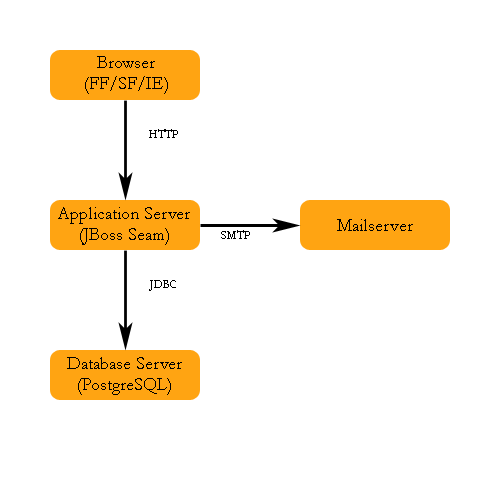
\includegraphics[scale=0.8]{../../img/salesmen_architecture.png}
\caption{Salesmen Architecture}
\end{figure}

\begin{figure}
\section{Infrastructure}
\label{fig_infrastructure}
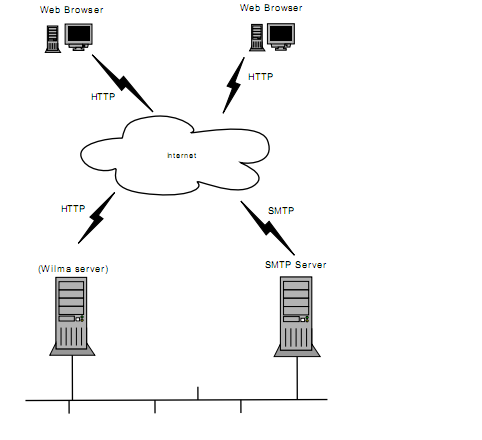
\includegraphics[scale=0.8]{../../img/infra1.png}
\caption{Salesmen infrastructure}
\end{figure}

\begin{figure}
\section{Modules}
\label{fig_modules}
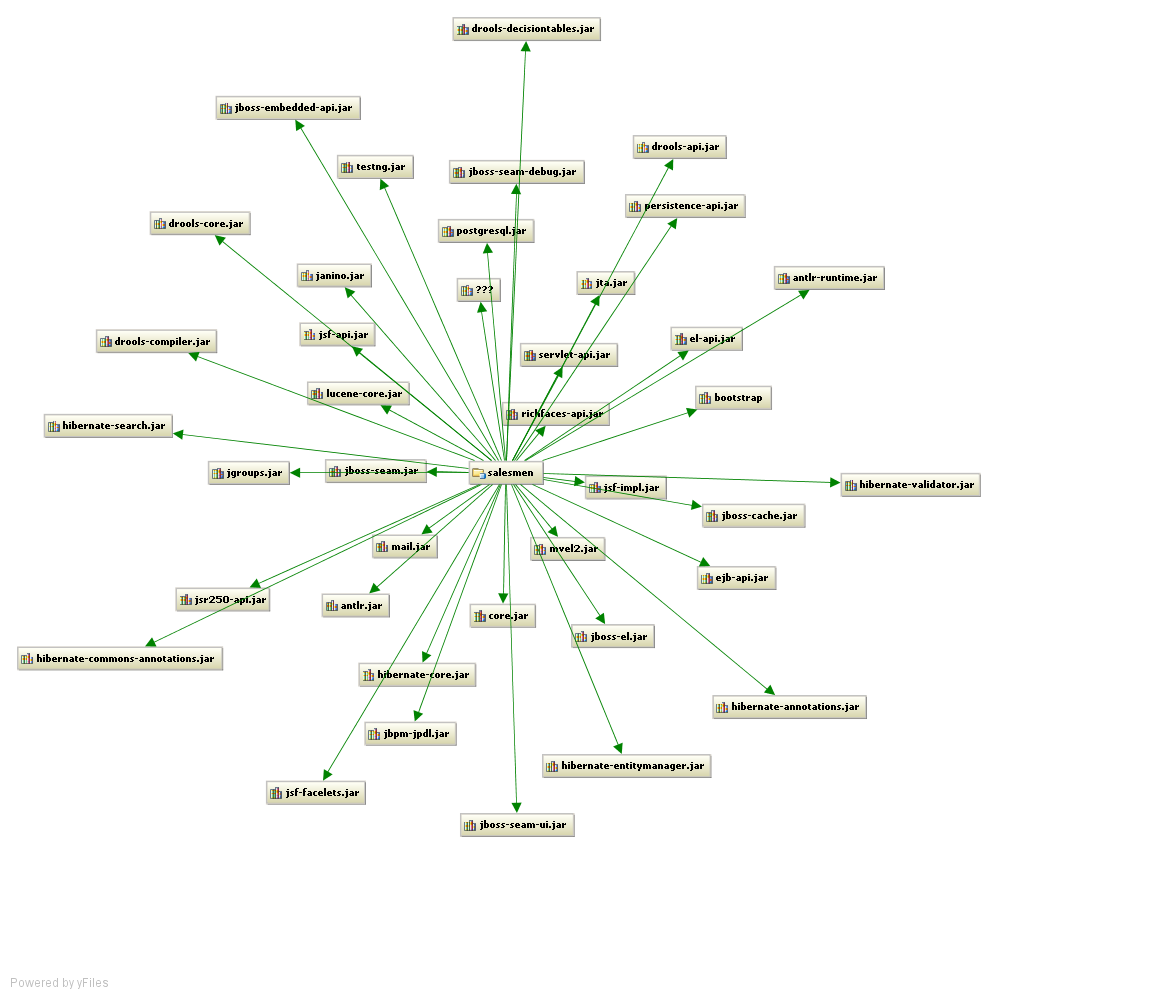
\includegraphics[scale=0.5]{../../img/salesmen_modules.png}
\caption{Salesmen - used modules}
\end{figure}

\begin{figure}
\section{Package Diagram}
\label{fig_package_entity}
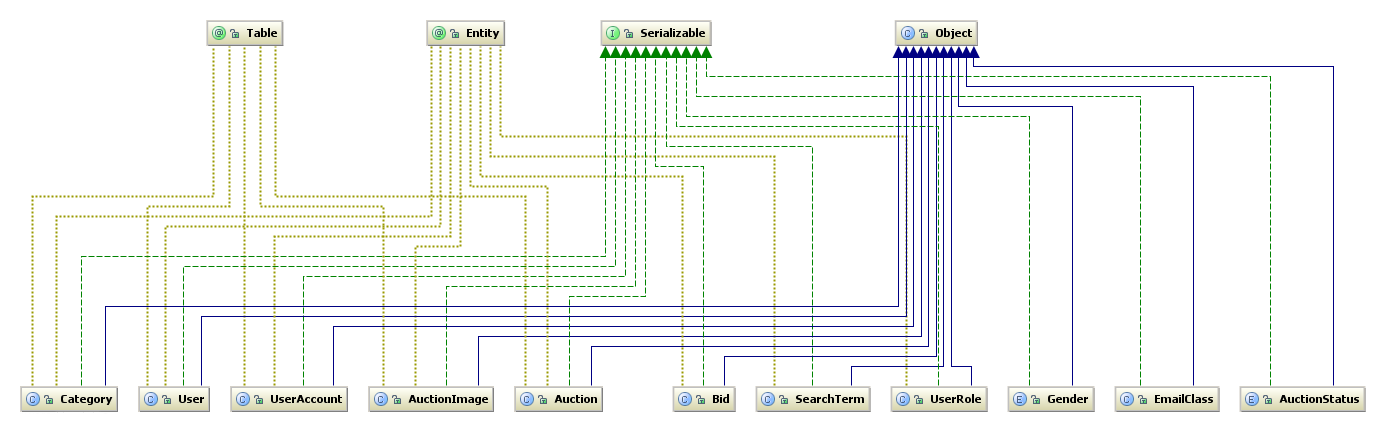
\includegraphics[scale=0.4,angle=90]{../../img/salesmen_package_entity.png}
\caption{Salesmen package diagram - global view}
\end{figure}

\clearpage
\begin{figure}
\section{Class Diagram - Entity package}
\label{fig_class1}
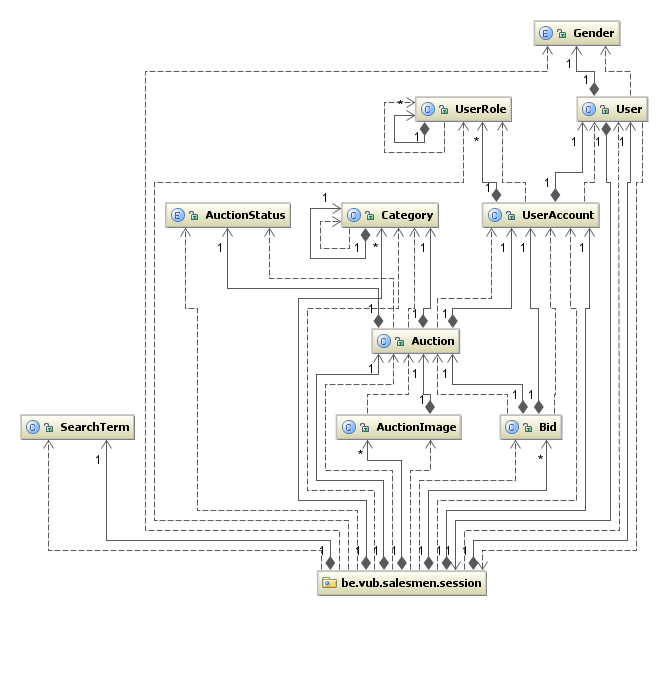
\includegraphics[scale=0.5]{../../img/salesmen_class_entity.png}
\caption{Salesmen class diagram - entity package expanded, session package collapsed}
\end{figure}

\begin{figure}
\section{Class Diagram - Session package}
\label{fig_class2}
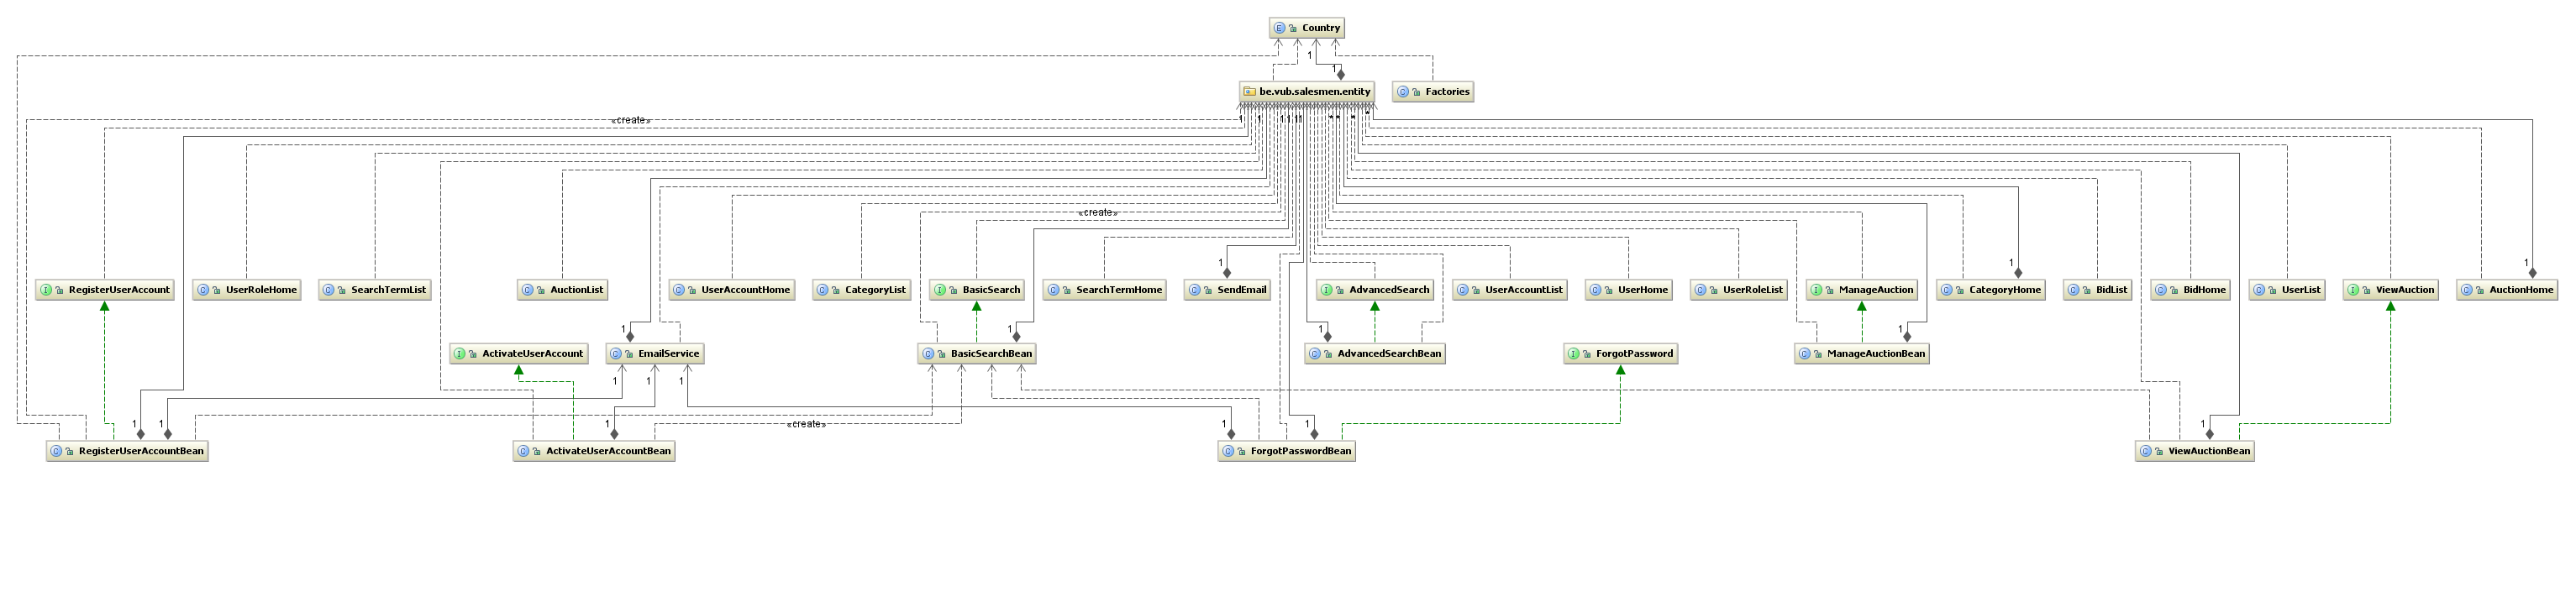
\includegraphics[scale=0.20,angle=90]{../../img/salesmen_class_session.png}
\caption{Salesmen class diagram - session package expanded, entity package collapsed}
\end{figure}

\begin{figure}
\section{Class Diagram - All packages}
\label{fig_class3}
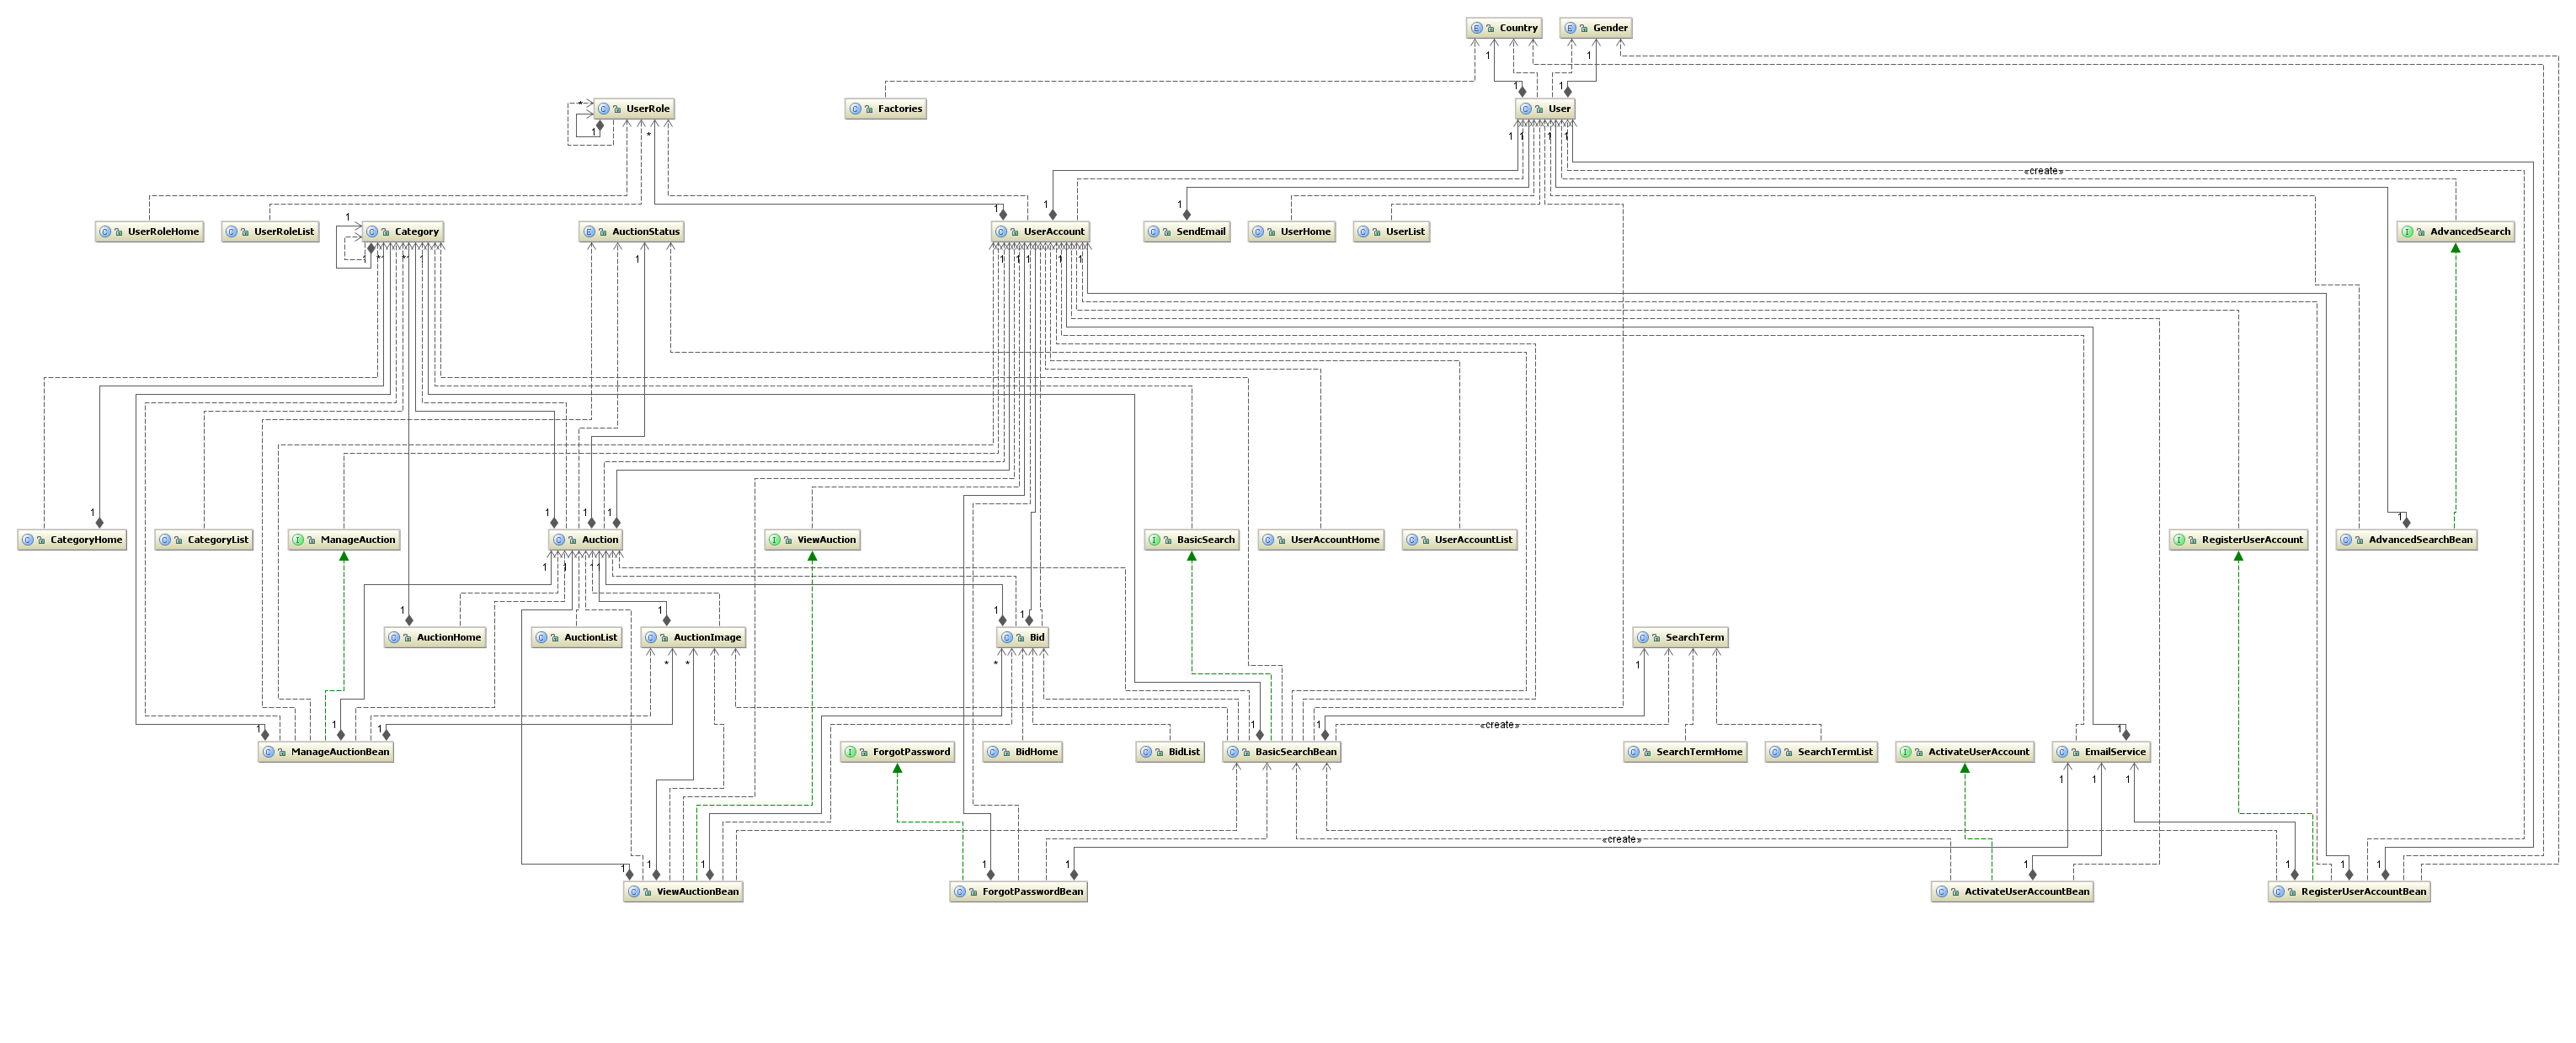
\includegraphics[scale=0.20,angle=90]{../../img/salesmen_class_all.png}
\caption{Salesmen class diagram - session and entity packages expanded}
\end{figure}

\clearpage
\begin{figure}
\section{Database diagram}
\label{fig_database}
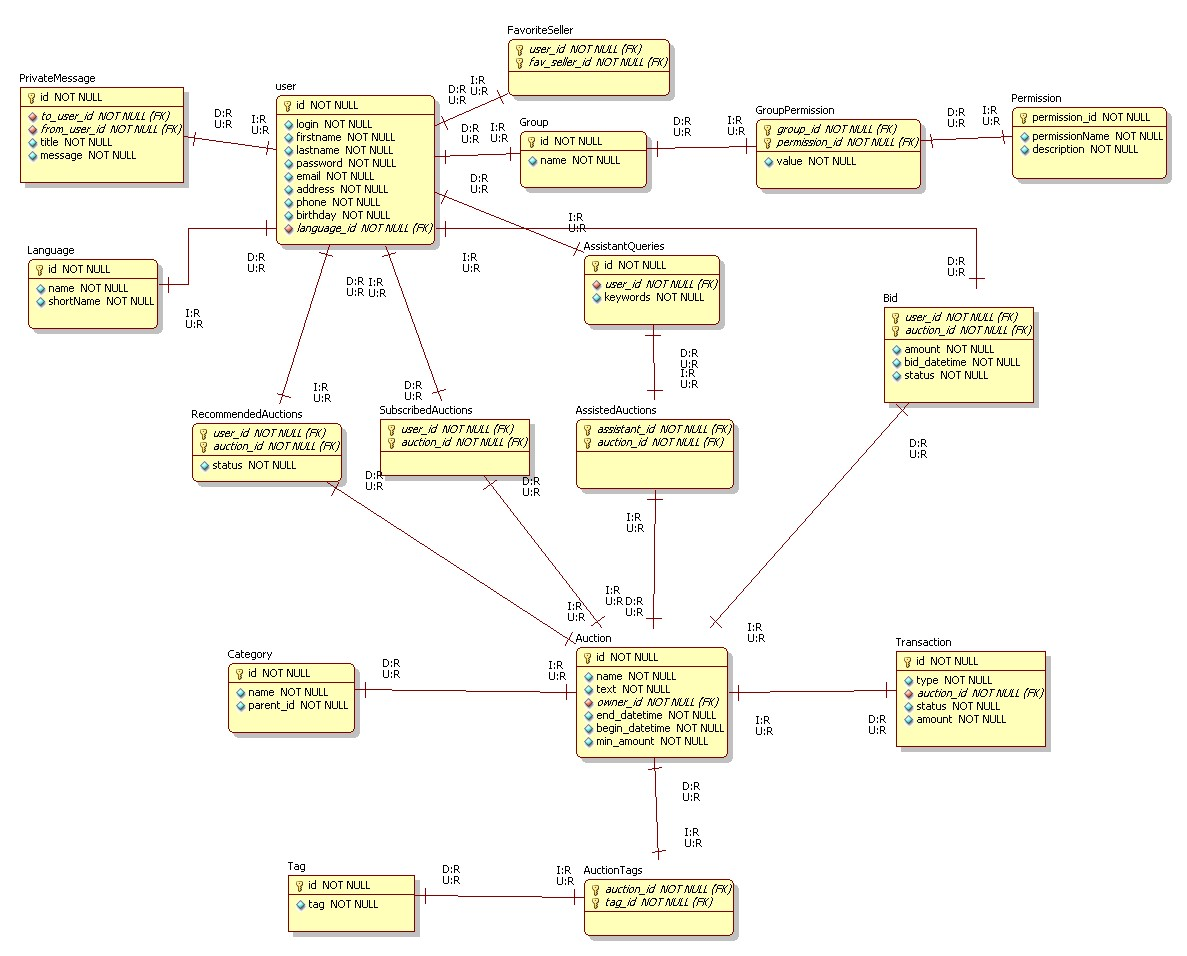
\includegraphics[scale=0.44,angle=90]{../../img/erd1.jpg}
\caption{Salesmen database layout}
\end{figure}

\chapter{Website Prototypes}
\begin{figure}
\section{Auction list}
\label{fig_prototype_auctionlist}
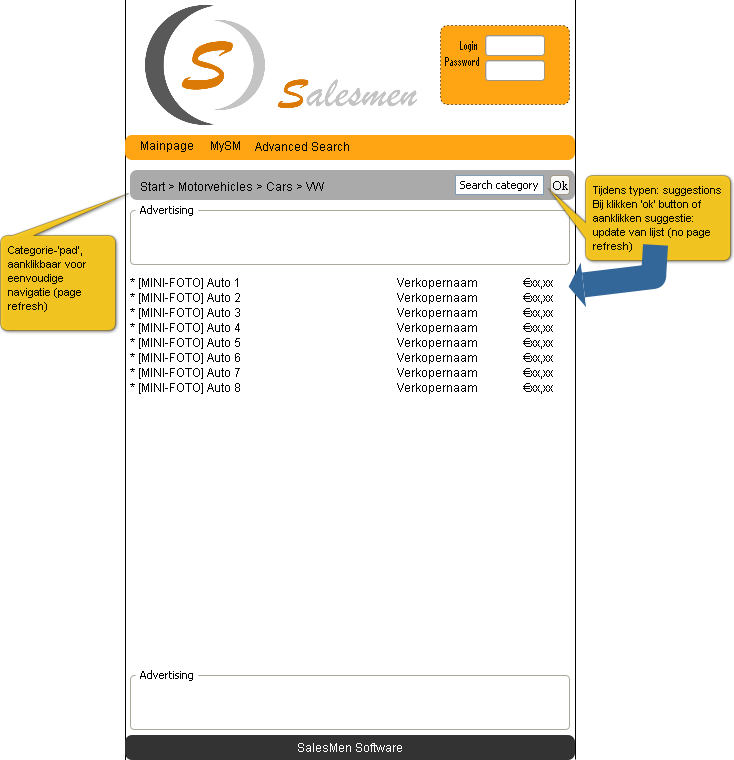
\includegraphics[width=15cm]{../../img/SM_auction_list.png}
\caption{auctionlist.seam}
\end{figure}
\begin{figure}
\section{Auction detail}
\label{fig_prototype_auctiondetail}
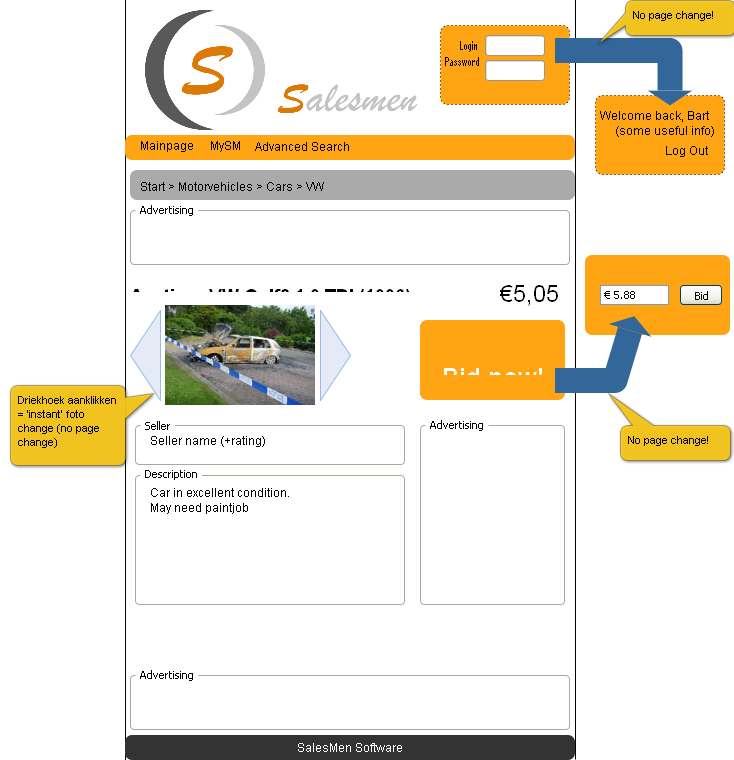
\includegraphics[width=15cm]{../../img/SM_auction_detail.png}
\caption{auction.seam}
\end{figure}
\begin{figure}
\section{Profile - Auctions}
\label{fig_prototype_profile_auctions}
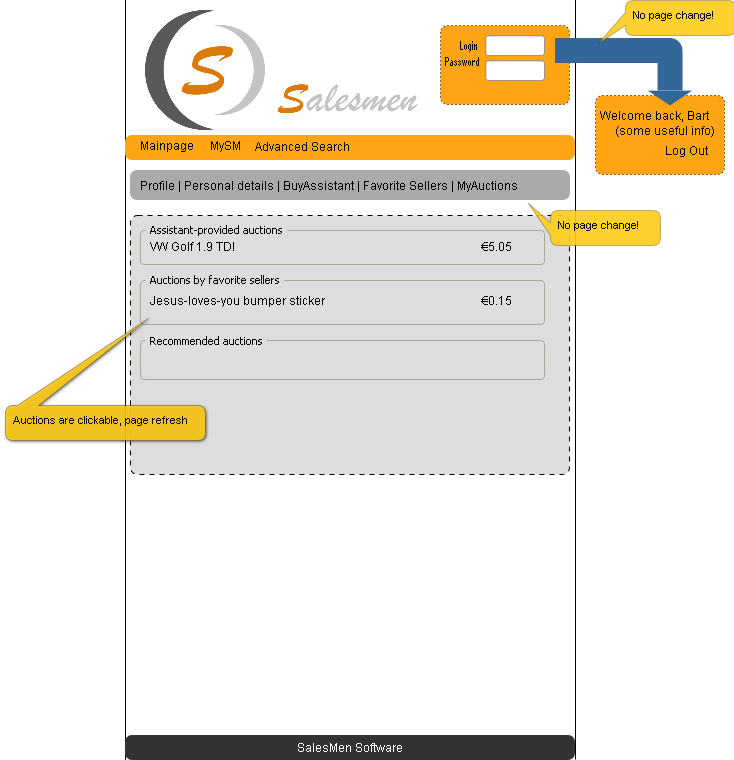
\includegraphics[width=15cm]{../../img/SM_mySM_auctions.png}
\caption{*.seam - auctions}
\end{figure}
\begin{figure}
\section{Profile - Buyers assistant}
\label{fig_prototype_buyer_assistant}
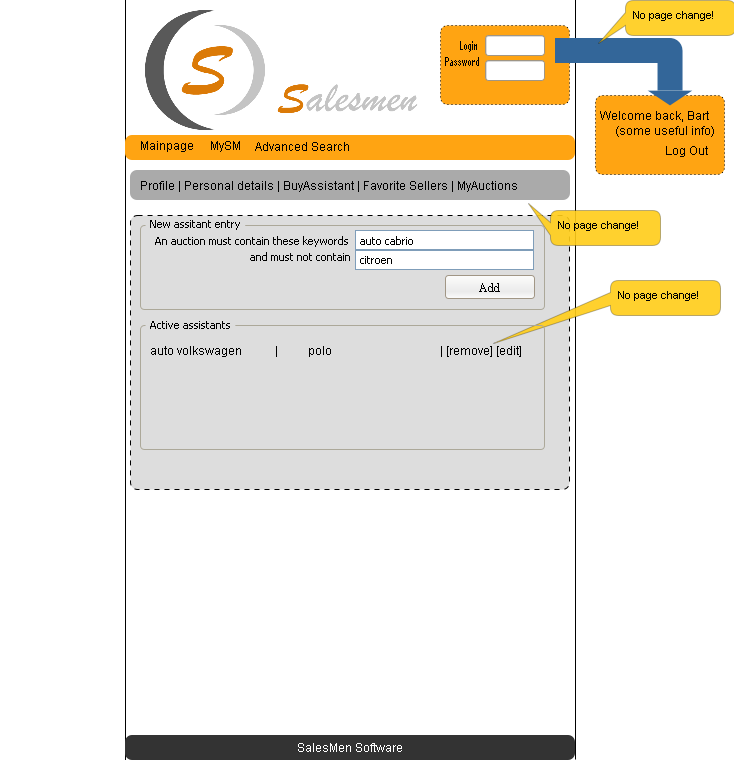
\includegraphics[width=15cm]{../../img/SM_mySM_buy_assistant.png}
\caption{*.seam - buyers assistant}
\end{figure}
\begin{figure}
\section{Profile - Personal information}
\label{fig_prototype_personal_info}
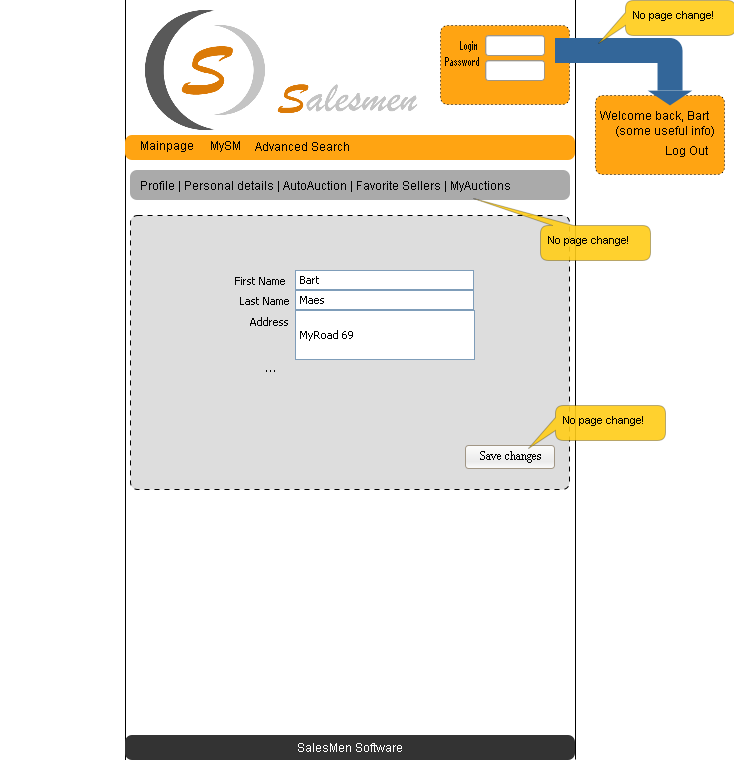
\includegraphics[width=15cm]{../../img/SM_mySM_personal.png}
\caption{*.seam - personal information}
\end{figure}
\begin{figure}
\section{Profile - Account information}
\label{fig_prototype_account_info}
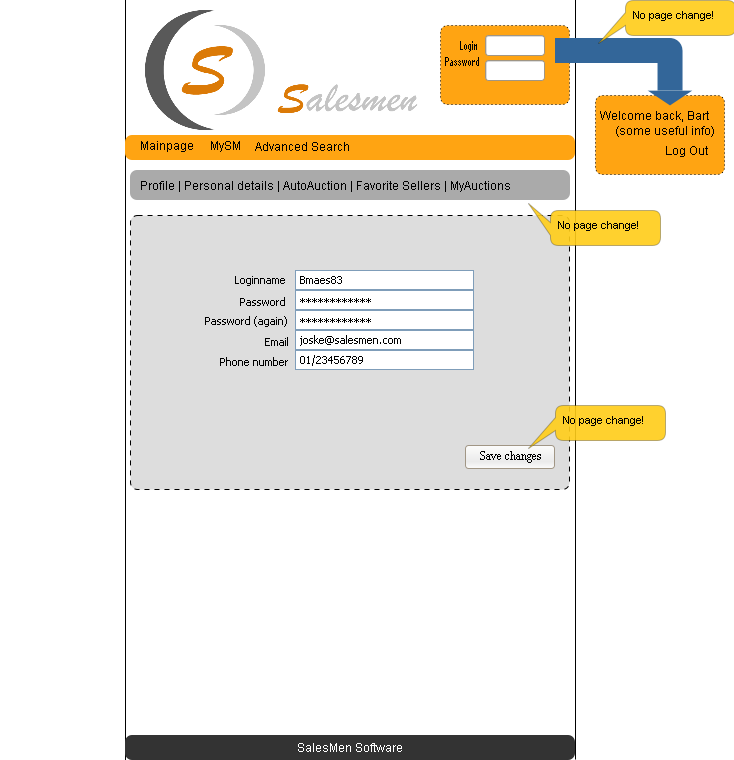
\includegraphics[width=15cm]{../../img/SM_mySM_profile.png}
\caption{*.seam - website information}
\end{figure}

\end{projdoc}
\end{document}
